%-------------------------------------------------------
\section{Introdução}
%-------------------------------------------------------


%-------------------------------------------------------
    \begin{frame}{Teoria Moderna de Portfólio e Índice Sharpe}
        
        \LARGE \textbf{Teoria moderna de portfólio \cite{markowitz1952portfolio}.}

        \Large
        % side by side text and figure
        \begin{columns}
            \begin{column}{0.5\textwidth}
                \begin{itemize}
                    \item Gestão de investimentos \cite{sethi2021nobel}.
                    \item Risco e retorno \cite{sharpe1964capital}.
                    \item Diversificação e preferência \cite{lintner1965valuation}.
                    \item Prêmio por unidade de risco \cite{sharpe1994sharpe}.
                \end{itemize}

            \end{column}
            \begin{column}{0.5\textwidth}
                \begin{figure}
                    \centering
                    \caption{Fronteira eficiente e Linha de Mercado}
                    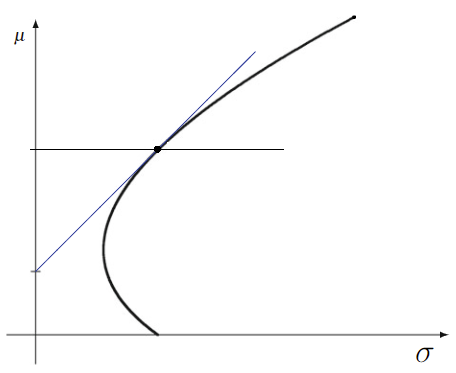
\includegraphics[width=0.6\textwidth]{images/fronteira_eficiente.png}
                    \par \footnotesize Fonte: adaptado \citeauthor{mansini2015linear}.
                \end{figure}
            \end{column}
        \end{columns}
        

    \end{frame}
    \note{    

        \ipar O mercado financeiro gerencia trilhões de dólares com uso da teoria moderna de portfólios elaborada pelo laureado do prêmio Nobel de economia Harry Markowitz \cite{sethi2021nobel}. As discussões sobre a teoria foram aprofundadas pelo também laureado William Sharpe, que aborda a estratégia de maximização de uma carteira de investimentos, considerando tanto o risco quanto o retorno. 
                
        \ipar A intuição do investidor seria que a máxima diversificação para um retorno esperado da carteira geraria um portfólio de mínima variância, isto é, com menor risco. Contudo, esta hipótese é rejeitada segundo a teoria de \citeonline{markowitz1952portfolio}, pois existe uma combinação ideal de ativos que compõem uma carteira de forma eficiente maximizando o retorno com o menor nível de risco. Portanto, a cada retorno esperado há uma combinação eficiente dos ativos que gera uma carteira de mínima variância, assim formando uma fronteira eficiente de combinações de ativos.

        \ipar A escolha da carteira eficiente é feita com base na relação entre risco e retorno. Segundo \citeonline{sharpe1964capital}, os investidores exigem um prêmio de retorno para assumir riscos adicionais. Desta maneira, a preferência dá-se pela aceitação ao risco, em que para opções de investimentos com o mesmo retorno esperado, o investidor escolherá a opção com menor risco \cite{lintner1965valuation}.

        \ipar Este prêmio por unidade de risco é conhecido como o índice Sharpe \cite{sharpe1994sharpe}. O termo foi apresentado por \citeonline{treynor1973use} em reconhecimento as contribuições feitas na avaliação de desempenho de fundos feita por \citeonline{sharpe1966mutual}, e atualmente é uma das medidas mais utilizadas para avaliação de desempenho de carteiras de investimento.

        \ipar Considerando que existe a opção para o investidor realizar empréstimo ou tomar emprestado a uma taxa livre de risco, é possível construir uma carteira eficiente que combina o empréstimo com todos os investimentos disponíveis no mercado. Esta combinação forma uma linha reta que tangencia a fronteira eficiente de ativos. Esta linha é denominada linha do mercado de capitais, e a carteira eficiente que tangencia a linha é chamada de carteira de mercado, que apresenta o maior prêmio por unidade risco \cite{sharpe1964capital}.

    }
%-------------------------------------------------------



%-------------------------------------------------------
    \begin{frame}{Séries Temporais e Redes Neurais}

        \LARGE \textbf{Otimização de Carteiras de Investimentos}

        \vspace{1cm}


            % side by side text and figure
            \begin{columns}
                \begin{column}{0.5\textwidth}
                    
                    \LARGE \textbf{Modelos Tradicionais \cite{zhou2023twostage}}

                    \Large
                    \begin{itemize}
                        \item Métodos estatísticos.
                        \item Séries temporais lineares.
                        \item \textit{ARIMA}.
                    \end{itemize}
                    \vspace{11pt}

                \end{column}
                \begin{column}{0.5\textwidth}
                    \LARGE \textbf{Novos Estudos}

                    \Large
                    \begin{itemize}
                        \item Aprendizado de máquina.
                        \item Séries temporais não lineares.
                        \item Redes neurais.
                        \item \textit{LSTM}.
                    \end{itemize}
                            
                \end{column}
            \end{columns}
            


    \end{frame}
    \note{
        
        Modelos Tradicionais -> Não linearidade -> Redes Neurais
        
        \ipar Uma estratégia de construção de carteira de investimentos é a otimização do índice Sharpe, que consiste em maximizar o índice Sharpe para uma carteira de ativos para obter a carteira de mercado \cite{maree2022balancing}. Para a otimização da carteira é necessário estimar o retorno e o risco da carteira. A estimativa do retorno esperado é feita com base em dados históricos, e o risco é estimado com base na matriz de correlação dos ativos e a volatilidade de cada ativo.

        \ipar Modelos de otimização também combinam previsão das séries temporais para estimar o retorno esperado da carteira. Modelos tradicionais de previsão de séries temporais, aplicam métodos estatísticos que consideram as séries como modelos lineares \cite{zhou2023twostage}. Dentre estes há os modelos de médias móveis auto-regressivas integradas (\acrshort{ARIMA}, do inglês \textit{Autoregressive Integrated Moving Average}), e heterocedasticidade condicional autoregressiva generalizada (\acrshort{GARCH}, do inglês \textit{Generalized Autoregressive Conditional Heterocedasticity}). 
        
        \ipar Entretanto, séries temporais de ativos financeiros como ações, apresentam uma dinâmi-ca de processo não linear. Há diversas abordagens para capturar dados não lineares, dentre estes há as redes neurais artificiais, modelos de redes neurais profundas, ou a rede neural recorrente que se provaram como ferramentas válidas para aplicações para dados de séries temporais multivariada \cite{cao2020delafo}. Além disso, os modelos podem ser combinados com métodos de otimização para a seleção de carteiras de investimentos \cite{du2022mean}.

        \ipar A aplicação de modelos de redes neurais com intuito de selecionar ativos para carteiras de investimentos é uma área que tem atraído a atenção de pesquisadores. O índice Sharpe tem sido utilizado em estudos como a função objetivo para a otimização de carteiras de investimentos com modelos de redes neurais \cite{tran2023optimizing}. Além disso, estuda-se a aplicação de redes neurais para predição do maior índice Sharpe no futuro \cite{vukovic2020neural}.

        \ipar Em geral, as redes neurais recorrentes (\acrshort{RNN}, do inglês \textit{Recurrent Neural Network}) têm se mostrado eficientes para previsão de séries temporais de ações \cite{wang2020portfolio}, em especial memória de longo prazo com curto prazo (\acrshort{LSTM}, do inglês \textit{Long Short-Term Memory}). Estes modelos de redes neurais utilizam uma camada de memória que permite a rede aprender dependências de longo prazo, e são capazes de capturar padrões de séries temporais não lineares para realizar previsões \cite{hochreiter1997long}.

        \ipar Há a possibilidade de combinar estruturas de redes neurais entre si para obter melhores resultados. O mecanismo de atenção tem sido efetivamente aplicado na área de processamento de linguagem natural, tem sido utilizado para melhorar o desempenho de modelos de redes neurais para previsão de séries temporais. Como exemplo, \citeonline{sun2022deep} desenvolveu um modelo para as séries temporais que combina uma rede neural convolucional com um transformador (rede neural baseada no mecanismo de atenção) para otimização de uma carteira de investimentos com objetivo de maximização do índice Sharpe.


    }
%-------------------------------------------------------





%-------------------------------------------------------
    \begin{frame}{Otimização e Redes Neurais}

        \LARGE \textbf{Otimização de Carteiras de Investimentos com Índice Sharpe}

        Combinação de redes neurais e otimização:

        \begin{itemize}
            \item \citeauthor{vukovic2020neural}(\citeyear{vukovic2020neural}): Perceptron multicamada para predição de ETF com melhor Índice Sharpe.
            \item \citeauthor{sun2022deep}(\citeyear{sun2022deep}): Redes Convolucionais com Atenção para otimização de carteiras por reforço com índice Sharpe.
            \item \citeauthor{cao2020delafo}(\citeyear{cao2020delafo}): Redes Recorrentes com Atenção para otimização de carteiras por reforço com índice Sharpe.
        \end{itemize}
                    

    \end{frame}
    \note{
        
        Combinação, complexidade e restrições reais

        \ipar Há a possibilidade de combinar estruturas de redes neurais entre si para obter melhores resultados. O mecanismo de atenção tem sido efetivamente aplicado na área de processamento de linguagem natural, tem sido utilizado para melhorar o desempenho de modelos de redes neurais para previsão de séries temporais. Como exemplo, \citeonline{sun2022deep} desenvolveu um modelo para as séries temporais que combina uma rede neural convolucional com um transformador (rede neural baseada no mecanismo de atenção) para otimização de uma carteira de investimentos com objetivo de maximização do índice Sharpe.

        \ipar Em modelos de otimização há restrições e parâmetros que podem ser adicionados para tornar o problema próximo ao real. \citeonline{mulvey2020optimizing} propõe um modelo de otimização de carteira de investimentos com redes neurais que considera a taxa de transação. 
        
        \ipar A aplicação de restrições como a taxa de transação, limitação de capital, e restrições como a de cardinalidade, que limita o número de ativos na carteira tornam o problema próximo da realidade, contudo aumentam a complexidade de resolução \cite{aithal2023real}. Uma abordagem para resolução de problemas complexos é a utilização de métodos heurísticos, que são métodos de busca que não garantem a solução ótima, mas são capazes de encontrar soluções próximas da ótima em um tempo computacionalmente viável \cite{milhomem2020analysis}.

        \ipar Os estudos sobre otimização de carteiras de investimentos pelo índice Sharpe têm apresentado somente uma restrição real, o efeito do custo de transação. Em maioria negligenciam questões como lote padrão, a aversão ao risco e outras restrições afetam a decisão sobre a alocação de ativos. Estes parâmetros seguem as regulações e práticas exercidas no mercado em que se inserem.

        \ipar O índice Bovespa (\acrshort{IBOVESPA}) é o principal indicador de desempenho das ações do mercado de capitais brasileiro e referência para investidores, reunindo as empresas mais importantes do mercado nacional. A composição do ativo é construída com base nos seguintes critérios: quanto ao volume financeiro no mercado a vista, quanto índice de negociabilidade e presença no pregão, e quanto ao valor do ativo \cite{B32023}. 

    }
%-------------------------------------------------------


%-------------------------------------------------------
    \begin{frame}{Objetivos}

        \Large 

        Avaliação da aplicação de redes neurais para previsão de índice Sharpe para seleção de carteiras de investimentos
    
        \begin{itemize}
            \item Revisão sistemática.
            \item Ferramenta para coleta de dados.
            \item Modelo de alocação incluindo parâmetros reais.
            \item Estruturas de redes neurais.
            \item Analisar o desempenho da seleção. 
        \end{itemize}


    \end{frame}
    \note{
            
        \ipar Este processo é complexo e demanda tempo e conhecimento do investidor. A aplicação de modelos de redes neurais para previsão de índice Sharpe pode auxiliar o investidor a tomar decisões de alocação de ativos, e a prever o desempenho de sua carteira de investimentos. 

        \ipar Logo, a contribuição deste trabalho é o desenvolvimento de uma ferramenta de seleção de carteiras de investimentos com a construção de um fluxo de processamento que permita o investidor obter uma carteira de investimento para a sua realidade, com base em um modelo de risco e retorno, e com a aplicação de redes neurais para previsão de índice Sharpe. 

        \ipar O objetivo principal deste trabalho é desenvolver e analisar uma estrutura que aplica redes neurais para previsão de índice Sharpe para seleção de carteiras de investimento.

        \ipar Para o desenvolvimento e análise de modelos seleção de carteiras de investimento, é necessário avaliar as referências historicamente mais relevantes e identificar estudos recentes sobre o tema. A partir da revisão bibliográfica, é possível identificar os métodos utilizados para construção de carteiras. Assim, busca-se identificar as tecnologias referentes a avaliação de risco e retorno para construção de carteiras de investimentos, identificar as técnicas de otimização para previsão de índice Sharpe e as estruturas de redes neurais para seleção de carteiras.

        \ipar A construção dos modelos são dependentes de dados históricos de ativos financeiros e dados de mercado. Portanto, é necessário a coleta de dados históricos de ativos financeiros e dados econômicos de forma estruturada e com qualidade de dados. Além disso, há a preocupação de tratamento e preparação dos dados, devido a não padronização das diferentes fontes.

        \ipar A partir da construção dos modelos, é necessário avaliar o desempenho da seleção de carteiras de investimentos. Para isso, o processo tem duas etapas principais: a otimização de carteiras de investimentos pela maximização do índice Sharpe, e a seleção da carteira de investimentos com base em redes neurais pela previsão de índice Sharpe. 

        \ipar A primeira etapa incorpora a construção de carteiras de investimentos com base em modelos de risco e retorno. Busca-se avaliar a  aplicação de parâmetros reais, como capital investido, custo de transação, rebalanceamento, lotes padrão, aversão a risco e cardinialidade. Para resolução, avalia-se métodos de otimização de programação não linear. Contudo, dado a complexidade do problema, faz-se necessário a avaliação de método heurístico para resolução.

        \ipar A segunda etapa incorpora a construção de redes neurais para previsão de índice Sharpe. Para isso, busca-se avaliar diferentes estruturas de redes neurais afim de identificar a que melhor se adequa ao problema. Estas redes passam por etapas de treinamento e validação com objetivo de avaliar o desempenho da rede neural.

        \ipar Por fim, avalia-se o desempenho da seleção de carteiras de investimentos aplicados a este fluxo de processamento de duas etapas. Portanto, seguindo as etapas descritas, de revisão, coleta, modelagem e análise tem-se a avaliação da aplicação de redes neurais para previsão de índice Sharpe para seleção de carteiras de investimentos.



        \begin{enumerate}
            \item Realizar uma revisão sistemática da literatura sobre seleção de carteiras de investimentos, com base em modelos de risco e retorno, e com base em redes neurais.
            \item Construir ferramenta para coleta de dados históricos de ativos financeiros e dados econô-micos de forma estruturada e com qualidade de dados.
            \item Desenvolver um modelo de alocação de ativos baseado no cálculo do índice Sharpe e com base em modelos de risco e retorno incluindo parâmetros reais.
            \item Elaborar estruturas de redes neurais para previsão de índice Sharpe e seleção da melhor carteira de investimentos.
            \item Analisar o desempenho da seleção de carteiras de investimentos aplicados a este fluxo de processamento de duas etapas. 
        \end{enumerate}


    }
%-------------------------------------------------------

